\section{Own Computations}\label{Own_computations}
This section presents my own computations I made to evaluate the Neural Stochastic Dual Dynamic Programming approach, specifically $v$-SDDP. 
In the following I will compare the $v$-SDDP approach with the standard SDDP approach with respect to computation time and present advantages and disadvantages of this novel approach.

The problem to benchmark these two approaches is the well known news-vendor problem.
I chose the news-vendor problem to conduct my computations, since it is a simple model that can be computed easily and even has an analytical solution. \\
The classical news-vendor problem is divided into two stages.
In the first stage, an agent wants to purchase a commodity that he can then sell in the second stage.
However, the agent does not know the demand of the commodity, since it is random and he can only purchase in the first stage \cite{BirgeLouveaux}.
Furthermore, the purchasing amount in stage one is bounded by a scalar $u$.
In the second stage, he can sell his items with a price of $q$ and he can also recycle said items for a price of $r$ while $r < q$. \\
According to \cite{BirgeLouveaux}, the news vendor problem can be formulated as follows:
\begin{subequations}\label{newsvendor_stufe1}
    \begin{alignat}{3}
          &\min_x        &\quad& c^T x + \mathbb{E}_\xi \left[ Q(x,\xi(\omega))  \right]\\
          &\textrm{ s.t.}  &\quad& 0 \leq x \leq u,
    \end{alignat}
\end{subequations}
with
\begin{subequations}\label{newsvendor_stufe2}
    \begin{alignat}{4}
         Q(x,\xi(\omega)) := & \min_y        &\quad& -qy(\omega) - rw(\omega)  \\
                            & \textrm{ s.t.}&\quad& y(\omega) \leq \xi(\omega)\\
                            &               &\quad& y(\omega) + w(\omega) \leq x \\
                            &               &\quad& y(\omega), w(\omega) \geq0.
    \end{alignat}
\end{subequations}
If $\xi \sim F(\cdot)$ and $F(\xi \leq \omega)$ is some cumulative probability distribution function that describes the distribution of the random demand, according to \cite{BirgeLouveaux} this problem can be solved analytically  with
\begin{equation*}\label{NewsVendorFormel}
    x_{opt} = \begin{cases}
    0 & \frac{q - c}{q - r} < F(0)\\
    u & \frac{q - c}{q - r} > F(u)\\
    F^{-1}(\frac{q - c}{q - r}) & \text{otherwise}
    \end{cases}.
\end{equation*}
This is another reason why I chose the news-vendor problem to conduct my computations, as it is one of the few stochastic programs that can be easily solved analytically.

Since I needed an SDDP solver for my own computation, I used the Python package MSPPY that is available on GitHub \cite{SDDP_Solver_Paper}.
For my implementation of the neural network of $v$-SDDP I used the snippets that were supplied in the supplementary materials in the NSDDP paper.
These snippets did not work on their own, so I had to do elaborate augmentations, however they still provided the general structure of the neural net. \\
The code for MSPPY solver required augmentation as well, since the provided version on GitHub did not work out of the box on my machine and I needed additional functionalities, like the export of the value function cuts to a pandas DataFrame, that were not supplied in the provided implementation.

Due to the simple structure of the news-vendor problem, the space of the decision variables is only one-dimensional, so a projection to a lower-dimensional space is not necessary.
My computations are therefore focused on the restrictions of the general $v$-SDDP approach. \\
Furthermore, for simplicity, a discrete and uniform probability distribution is used to simulate the random demand.

In the beginning, I started by formulating the simple news-vendor problem shown in \ref{newsvendor_stufe1} - \ref{newsvendor_stufe2} with MSPPY and used the provided SDDP solver to solve this initial problem. \\
For the initial news-vendor problem, the first stage variable is upper bounded by 25, so $u=25$, the other coefficients where initialized as $c=1$, $q=2$, $r=0.5$ and for the probability distribution a discrete uniform distribution between $1$ and $10$ is used. \\
Using the SDDP solver, the algorithm converges after 6 iterations and approximately 3 seconds to an optimal solution.
The optimal amount of newspapers to buy is $7$, according to the SDDP solution.
Using the formula \ref{NewsVendorFormel}, the optimal amount is $F^{-1}(\frac{q-c}{q-r}) = F^{-1}(\frac{2}{3})=7$.
This quick example is assuring, as the used SDDP implementation is indeed working correctly.

Since $v$-SDDP is meant to be used in an online fashion, where similar problem instances are solved and the corresponding value function approximation is used to improve and speed up further approximations, data is necessary to train the neural network and to analyze the NSDDP approach.
I am in no environment where this kind of data is available, so I had to create my own data.

In order to accomplish this, I generated $10.000$ random samples for each of the parameters.
For the parameter $u$, which was the upper bound for the first stage solution, I generated discrete, uniform distributed random samples.
For the upper and lower bound of this random variable I chose $25 \pm 25\cdot 0.4$. \\
The rest of the parameters I generated $10.000$ normal distributed random samples and for the respective means I chose the parameters from the initial problem, so $c=1$, $q=2$, $r=0.5$, respectively.
The standard deviation for each random variable was set to $40\%$ of the mean.

For each of these samples I solved the corresponding problem instance, to check which parameter tuple generates a feasible optimization problem and also to use the respective data tuple and corresponding optimality cuts as a data point to train and test the neural net. \\
The tuple was of the form $(u, c, q, r, uncert)$, where $u$ represents the upper bound for the first stage decision, $c$ is the cost coefficient for the first stage objective function and $q$ and $r$ are the selling price and recycle price for the newspapers, respectively.
The $uncert$ is a representation of the used probability distribution. \\
Since I used a discrete, uniform distribution for the demand, this was equivalent to the right interval limit, since I used one as the left interval limit.
Out of the generated $10000$ data points, only 8444 were feasible points, which I used for the training and test sets.

In \cite{NSDDP} the neural network is designed in a way that the number of cutting planes to approximate the value function is a hyperparameter, i.e. needs to be determined before training. \\
Since the model uses a multi-layer perceptron to generate the approximations, the model can not deal with variable output dimensions.
This implies that either the generated cuts need have to be artificially enhanced by extending or cutting the dimension to the necessary output dimension or that only these generated samples are used that have the correct output dimension.
Since artificially enhancing the cuts can lead to unpredicted behavior, such as that optimal points would violate the enhanced cuts, I choose to only use the samples that have the necessary number of cuts and do not need augmentation.

This highlights the first downside of this approach, that the number of cuts is fixed to the chosen hyperparameter and hence limits the information content that can be embedded in the dataset. \\
In order to tackle this downside, \cite{NSDDP} proposes a solution, by introducing a learnable scalar that represents the number of cutting planes.
However, in the scope of this seminar paper, I chose to use a fixed number of linear cuts for the value function approximation for simplicity.

As a first step to see if the model I used worked correctly, I tried to predict the value function approximation using just a single data point.
If the model was correct, it should be able to perfectly approximate the data point. \\
Using the proposed model from \cite{NSDDP} that used an MLP with a hidden layer consisting of 128 neurons did not as well as expected, since it took about $200$ iterations by passing the training data all at once until the loss was under a threshold of $10^{-1}$. \\
My theory is that the network was too large for this small problem, since the intended problem class of this approach was much larger than this, hence a lot more neurons have to be trained to learn this one data point by heart.

I then changed the number of neurons in the hidden layer from 128 to just two. With this change, the data point could be perfectly predicted after $80$ training steps, which still seems quite a lot for this kind of small problem, but works better than the proposed 128 neurons.
As the model seemed to work, I increased the number of cuts to see how the network would react to this change.
This small change drastically presented a big disadvantage of this approach, as now the predicted cuts where causing the problem instances to be infeasible or that the SDDP algorithm was not able to converge on the problem instance.
Most likely the predicted cuts where not accurate enough and cut optimal points away or lead to degeneracy.

Since the neural network is just doing a regression and will always have some error, there is no guarantee that the network will always provide lower bounds on the value function approximation.
It can easily happen, that due to a small error in the coefficients for the linear-affine cut, the original optimal point becomes infeasible or the optimal point is removed with a cut from $v$-SDDP. 
I was able to resolve this issue by lowering the tolerance for the loss function from $10^{-1}$ to $10^{-4}$. \\
In general, I made the observation that the more pieces for the value function approximation are used, a lower tolerance for the loss-score is necessary to ensure feasibility to some degree.
Furthermore, my experiments made it clear that it is crucial to provide correct and meaningful data, since I had a few cases where the neural network did not converge on the training set, probably because there was not enough variation in the input data.

A further big change could be observed when lowering the learning rate or stepsize of the optimizer, as this change enabled the convergence on problems where the solver could not converge beforehand.
In the experiments that I conducted, the optimizer Adam \cite{adam_optimizer} worked better than the standard stochastic gradient descent algorithm. \\
As it is common practice to not train a model on the whole dataset at once, but on smaller batches of data, I choose to train the network with batches of size 32. \\
This specific batch size was chosen, since it is a common rule of thumb to use batches that size are a power of 2, usually 32 and 64 are used, and 32 seemed to work reasonably well.
This significantly reduced the number of necessary epochs to just four.

As my initial hyperparameters, I chose to predict two cuts for the news-vendor two stage problem and chose only one layer with 128 neurons in the hidden layer for the network.
The data was split in training and test set, whilst the test set was $30\%$ of the whole dataset. 

In figure \ref{fig:train_test_2pieces} the training and test loss is presented.
To calculate that loss, the objective function, hence the earth-mover distance, of the problem was used.

\begin{figure}[H]
    \centering
    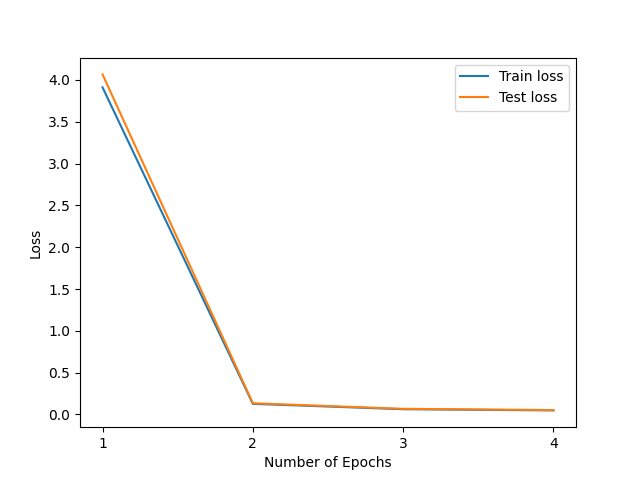
\includegraphics[width=0.85\linewidth]{correct_train_test_loss2piece.png}
    \caption{Train and test loss for the neural net to predict 2 cuts with one hidden layer consisting of 128 neurons.}
    \label{fig:train_test_2pieces}
\end{figure}

As it can be seen in figure \ref{fig:train_test_2pieces}, the performance on the training and test dataset is almost identical, meaning the model performs almost perfectly on the test set.\\
One reason for this behavior is probably due to the artificial nature of the data.
Since it performs so well on the unseen test set, I assume also good performance on completly new data.\\
After that, I trained the model on 8563 training tuples that created beforehand.
I wanted to compare the solution times for different hyperparameter combinations, so I trained multiple models.
These models were then benchmarked on samples from the test set to compare the respective computation times.

For all combinations I only used models with one hidden layer, since one was already sufficient to create good predictions and more would probably just overfit the data.
I tried multiple quantities of hidden neurons, aside from the proposed 128, and up to 110 hidden neurons the trained models were never able to solve every presented problem instance, meaning that the predicted optimality cuts lead to infeasibility or cycling of the solver.
Because of that, I only looked at models with 128 hidden neurons. \\
The hyperparameter left to vary was the number of cutting planes that the neural network predicts.
As the representation of the problem instance is 5-dimensional, it is not expected that the network is able to reliably predict more than two cuts, since each cut consists of two coefficients, if the decision variable is one-dimensional, so for two cuts four coefficients are needed. \\
This implies that the model should only be able to predict two optimality cuts.
Of course, this is only the case if the coefficients are independent of each other, which is probably does not hold.
Because of that, I also chose to look at the results for three predicted cuts.

For each hyperparameter, the training and test data had to be trimmed in order to provide uniform output dimensions, since the neural network can not deal with a variable number of output dimensions.
This lead to an effective reduction of the dataset size by about 10 to 20 samples. 
For each hyperparameter configuration, the respective model was trained and used to predict optimality cuts on five randomly selected instances from the test set.
These instance were solved by using the standard SDDP algorithm and the $v$-SDDP algorithm.
The comparison of the respective solution times is visualized in figure \ref{fig:Solution Comparison}.
\begin{figure}[h]
    \centering
    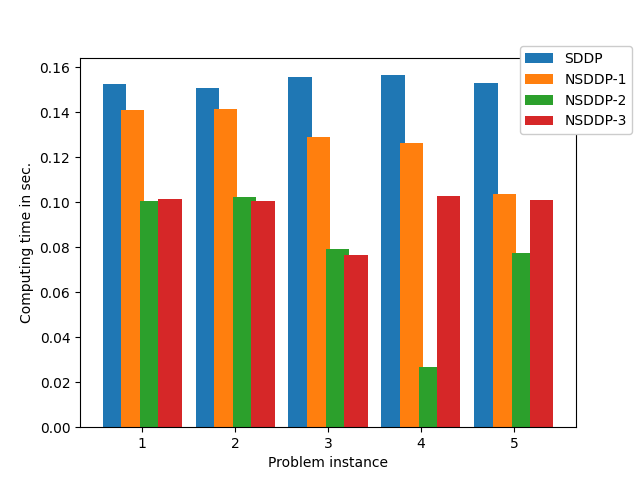
\includegraphics[width=\linewidth]{Computing_comparison_128hidden_neurons.png}
    \caption{Comparison of computing time on five random problem instances from the test data set. SDDP describes the solution time of the standard SDDP algorithm. NSDDP-1 describes the computing time of $v$-SDDP with one predicted cutting plane}
    \label{fig:Solution Comparison}
\end{figure}

It is clear from figure \ref{fig:Solution Comparison} that more predicted optimality cuts provide better computation times.
An interesting comparison is between the computation time of $v$-SDDP with two and three optimality cuts, respectively. \\
In general, it would seem that the more cutting planes are predicted, the lower the computation time.
However, as seen in problem instance four and five, the model with just two cutting planes is substantially faster than the one with three cutting planes. \\
Since the solution with two cutting planes in instance four is computed almost instantly, it can be assumed that the cutting planes provided from $v$-SDDP in this instance are all the cutting planes that are needed to compute an optimal solution.
The three generated cutting planes possess less predictive power, as they have a longer computing time. \\
This could be the result of my argument that in my specific use case only the prediction of two optimality cuts should be applicable, since three cuts are too high-dimensional to reliable make predictions with this kind of network.
It seems that for some instances the approach with three cuts is able to achieve slightly better performance but is not able to generalize that on all instances.

It could be shown that the NSDDP approach can lead to an acceleration of the computing time of $30-40\%$ on average using more than one cutting plane.
However, the used two-stage news-vendor problem instances are very small problem and the neural network still needed 128 neurons in the hidden layer, which indicates that this approach needs a lot of resources.
